\chapter{راهنمای نصب}
سند حاضر،‌ حاوی مراحلی است که برای نصب و راه‌اندازی سیستم برنامه‌ریزی منابع سازمان لازم است طی شود.

\newpage
\section{نیازمندی‌های سیستم}
نصب سیستم برنامه‌ریزی روی هر یک از سیستم‌های عامل ویندوز، لینوکس و 
\lr{OS X}
امکان‌پذیر است. در ادامه، مراحل نصب تشریح شده است.

\begin{enumerate}
	\item نصب JRE8 یا همان
	\lr{Java Runtime Environment} 
	: در ابتدا نسخه‌ی ۸ (یا بالاتر) از JRE را از نشانی زیر بارگیری و نصب نمایید. توجه داشته باشید که لازم است نسخه‌ای را بارگیری کنید که با سیستم‌عامل شما سازگار باشد.\\
\url{http://www.oracle.com/technetwork/java/javase/downloads/jre8-downloads-2133155.html}\\
	
در صورتی که برای نصب JRE8 نیاز به راهنمایی بیشتری دارید به نشانی زیر مراجعه فرمایید.

\url{https://docs.oracle.com/javase/8/docs/technotes/guides/install/install_overview.html}\\

پس از اتمام نصب، می‌توانید با اجرای دستور java از موفقیت یا عدم موفقیت آن مطلع گردید. (شکل 
\ref{f12}
)

	\begin{figure}[H]
		\centering
		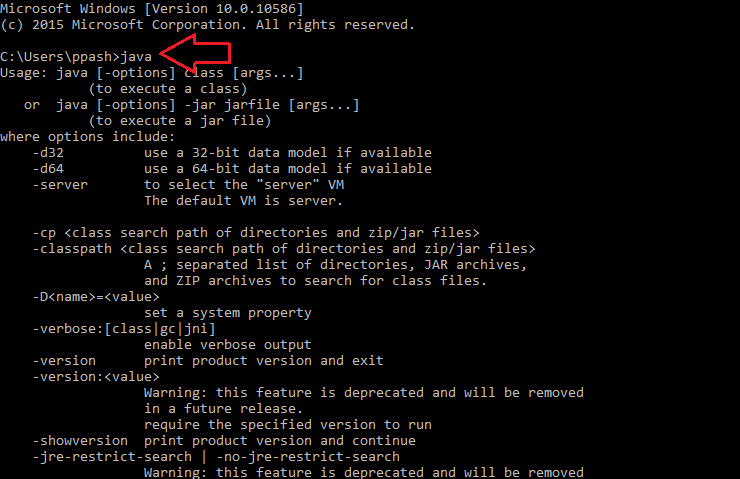
\includegraphics[scale=0.6]{img/install/java}
		\caption{نصب موفق JRE بر روی ویندوز}
		\label{f12}
	\end{figure}
	
	\item نصب کارگزار MySQL :
	ابتدا به نشانی زیر بروید و پرونده‌ی نصب کارگزار MySQL را بارگیری کنید.\\
\url{http://dev.mysql.com/downloads/mysql/}\\


در صورتی که برای نصب کارگزار MySQL نیاز به اطلاعات بیشتری دارید، به نشانی زیر مراجعه نمایید.\\
\url{http://dev.mysql.com/doc/refman/5.7/en/installing.html}\\

	پس از نصب آن، با اجرای دستور mysql در خط فرمان، از اجرای صحیح آن در سیستم خود اطمینان حاصل فرمایید.\\	\\	
	
	
	\item نصب xampp
	برای اینکه بتوانید از خدمات MySQL و Apache و PHP که برای نصب و استفاده از سیستم برنامه‌ریزی موردنیاز است استفاده نمایید، لازم است نرم‌افزار xampp را از نشانی زیر بارگیری و نصب نمایید.\\
\url{https://www.apachefriends.org/download.html}\\
	
	پس از نصب  xampp ،آن را اجرا کرده و خدمات Apache و MySQL را در آن فعال نمایید. در صورتی که فعال شدن موفقیت‌آمیز باشد، صفحه‌ی xampp به شکل
	\ref{f13}
	در خواهد آمد.
	
		\begin{figure}[H]
			\centering
			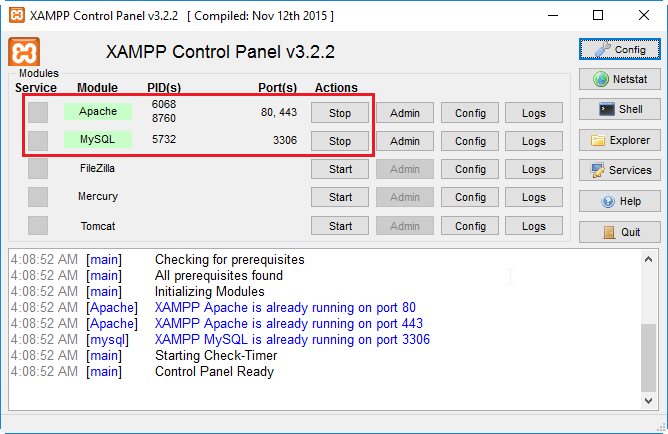
\includegraphics[scale=0.7]{img/install/xampp}
			\caption{xampp همراه با خدمات فعال}
			\label{f13}
		\end{figure}
		
		
	\item نصب نرم‌افزار اصلی: روی پرونده‌ای که در اختیار شما قرار گرفته است کلیک نمایید و مراحل را به صورتی که در پنجره‌ی باز شده می‌آید طی کنید.
سپس به محل نصب بروید و پوشه‌ی نصب شده را مشاهده نمایید. سپس پرونده‌هایی که با پسوند jar هستند (بجز فایل  ERP  ) در پوشه‌ای با نام lib قرار دهید. پرونده‌ای که شما اجرا می‌کنید، ERP.jar خواهد بود.

		
	\item راه‌اندازی پایگاه‌داده:
	پرونده‌های install\_db.php و erp\_db.sql را در نشانی وب php کپی نمایید. در صورتی که تنظیمات xampp را تغییر نداده باشید، این نشانی، 
	  C:\textbackslash{}xampp\textbackslash{}htdocs خواهد بود. حال install\_db.php را با ویرایشگر متنی موردعلاقه‌ی خود باز کنید. پیشنهاد ما، استفاده از
	\lr{Sublime Text}
	است. در چند خط ابتدای این پرونده، نام کاربری و رمز عبور mysql ای را که بر روی سیستم است وارد نمایید. (خطوط ۶ تا ۸)
	 سپس در مرورگر خود به نشانی
	localhost/install\_db.php
	بروید. با اجرای این پرونده php، پایگاه‌داده در سیستم شما راه‌اندازی و پیکربندی خواهد شد. در صورتی که عملیات موفقیت‌آمیز باشد با شکل 
	\ref{f15}
	مواجه خواهید شد.
			\begin{figure}[H]
				\centering
				
\includegraphics[scale=0.7]{img/install/db}
				\caption{راه‌اندازی موفقیت‌آمیز پایگاه‌داده}
				\label{f15}
			\end{figure}
	
	\item پیکربندی نرم‌افزار:
	در محل نصب نرم‌افزار، پرونده‌ی erp.conf را با ویرایشگر متن دلخواه خود باز کرد و مشخصات میزبان، پورت، نام کاربری و رمزعبور پایگاه‌داده را وارد نمایید. توجه نمایید که قالب این پرونده تغییر نکند. در شکل زیر، قالب کلی این پرونده قابل مشاهده است.
	
			\begin{figure}[H]
				\centering
				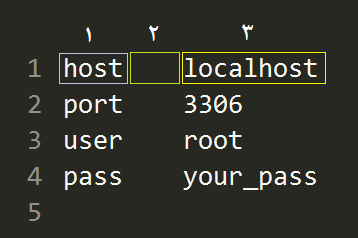
\includegraphics[scale=0.6]{img/install/conf}
				\caption{قالب پرونده‌ی پیکربندی}
			\end{figure}
	
	همانطور که مشاهده می‌نمایید، این پرونده دارای چهار سطر است که به ترتیب مربوط به میزبان، پورت، نام کاربری و رمزعبور مربوط به پایگاه داده است. هر سطر دارای دو بخش کلید (۱) و مقدار (۳) است که با یک فضای سفید (۲) تب
	\LTRfootnote{Tab}
	جدا شده‌اند. توجه کنید که این فضای سفید حتما باید از نوع تب باشد.\\
	در هر سطر، بخشی که شما تغییر می‌دهید، بخش ۳، یعنی «مقدار» است که در سطر اول با رنگ زرد مشخص شده است.\\
	پس از اعمال تغییرات، پرونده را ذخیره نمایید.
	
	
	
	\item اجرای سیستم برنامه‌ریزی: 
در صورتی که گام‌های پیشین درست طی شده باشند، با دو بار کلیک بر روی پرونده‌ی ERP.jar ، سیستم برنامه‌ریزی اجرا خواهد شد. در صورتی که نخستین بار باشد که از سیستم برنامه‌ریزی استفاده می‌کنید، با  شناسه‌ی
\lr{1}
  و رمز عبور admin وارد شوید. 
	
\end{enumerate}

\section{نصب بر روی سرور}
مراحلی که تا این‌جا شرح داده شد، جهت نصب، پیکربندی و استفاده از سیستم برنامه‌ریزی بر روی سیستم محلی است. برای اینکه از سرور (و به صورت غیر محلی) از سیستم استفاده کنید، نیازی به نصب کارگزار  MySQL بر روی سیستم محلی خود ندارید. همچنین، اکثر کارگزارها، دارای Apache ، PHP و  MySQL هستند. شما تنها کاری که باید انجام دهید، این است که نصب و پیکربندی پایگاه‌داده را روی کارگزار سازمان انجام دهید و در پرونده‌ی پیکربندی و در بخش  mysql\_host نشانی کارگزار سازمان را وارد نمایید و نرم‌افزار اصلی (ERP.jar) را اجرا نمایید.

